\documentclass[a4paper, 10pt, twoside, notitlepage]{article}

%idioma
\usepackage[spanish]{babel}
\usepackage[utf8]{inputenc}

% matematica
\usepackage{amsmath}
\usepackage{amsfonts}
\usepackage{amssymb}

% estilo
\usepackage[footnotesize]{caption}
\usepackage[outer=2cm,inner=4cm,top=2cm,bottom=2cm]{geometry}
\usepackage{fancyhdr}
\usepackage{listings}
\usepackage{pdfpages}
\usepackage{verbatim}
\usepackage{float}
\usepackage{svg}

\usepackage{color,hyperref}
\definecolor{black}{rgb}{0.0,0.0,0.0}
\definecolor{darkblue}{rgb}{0.0,0.0,0.3}
\definecolor{color_fondo}{rgb}{0.2, 0.2, 0.2}
\definecolor{color_fuente}{rgb}{0.8, 0.8, 0.8}
\definecolor{codegreen}{rgb}{0,0.6,0}
\definecolor{codegray}{rgb}{0.5,0.5,0.5}
\definecolor{codepurple}{rgb}{0.58,0,0.82}
\definecolor{backcolour}{rgb}{0.95, 0.95, 0.92}

%\lstdefinelanguage{C}
%{
%  morekeywords={from, import, def, return},
%  morecomment=[l]{//},
%  morestring=[b]",
%  alsodigit={-},
%  alsoletter={&}
%}

\lstdefinestyle{mystyle}{
	language=C,
    backgroundcolor=\color{color_fondo},   
    commentstyle=\color{codegreen},
    keywordstyle=\color{magenta},
    numberstyle=\tiny\color{codegray},
    stringstyle=\color{codepurple},
    basicstyle=\ttfamily\footnotesize,
    breakatwhitespace=false,         
    breaklines=true,  
    postbreak=\mbox{\textcolor{red}{$\hookrightarrow$}\space},               
    captionpos=b,                    
    keepspaces=true,                                  
    numbersep=5pt,                  
    showspaces=false,                
    showstringspaces=false,
    showtabs=false,                	  
    tabsize=2
}

\lstset{style=mystyle, 
		language=C, 
		literate={\ }{{\ \allowbreak}}{1},
		literate=
		{á}{{\'a}}1
		{é}{{\'e}}1
		{í}{{\'i}}1
		{ó}{{\'o}}1
		{ú}{{\'u}}1
		}

\hypersetup{colorlinks,breaklinks,linkcolor=black,urlcolor=darkblue,anchorcolor=darkblue,citecolor=darkblue}

% =============================================================================== %
% COLOR DE PÁGINA
% =============================================================================== %
\usepackage{pagecolor}

% Para usar fondo blanco y letra negra comentar los dos comandos que siguen
\color{color_fuente}
\pagecolor{color_fondo}

\pagenumbering{arabic}    % arabic, gobble

\pagestyle{fancy} % Encabezado y pie de página
\fancyhf{}
\fancyhead[L]{[66.20/86.37] Organización de Computadoras - 2do cuatrimestre 2022}
\fancyhead[R]{\hfill\includegraphics[width=2.5cm]{lhead.png}}
\renewcommand{\headrulewidth}{0.4pt}
\fancyfoot[C]{Página \thepage}
\renewcommand{\footrulewidth}{0.4pt}

\title{\textbf{Trabajo Práctico 0\\Infraestructura Básica} \\}

\author{ \\
         Melina Cheminet, \textit{Padrón 102123} \\
          \texttt{ mcheminet@fi.uba.ar }       \\
		  [2.5ex]
        \\
        Fernández Elfi, Facundo, \textit{89843} \\  \texttt{ffelfis@gmail.com}\\ 
		  [2.5ex]
		 \\
        David Batallan, \textit{Padrón 97529}     \\
          \texttt{dbatallan@fi.uba.ar}                      \\ 
		  [2.5ex]
		 \\
         \normalsize{2do. Cuatrimestre de 2022}            \\
         \normalsize{86.37 / 66.20 Organización de Computadoras} \\
         \normalsize{Facultad de Ingeniería, Universidad de Buenos Aires} 
       }

\date{22/09/2022}


\begin{document}
	
\maketitle
	
\begin{abstract}
El objetivo de este trabajo es familiarizarse con la herramienta QEMU que utilizaremos durante el curso. Con este fin se desarrollará un programa en C que resuelva el pedido de conteo de caracteres, palabras y líneas. Dicho programa también tendrá una documentación de ayuda para su uso. Se realizarán pruebas de funcionamiento y mediciones de tiempo de trabajo para la ejecución del programa.
\end{abstract}

\tableofcontents
\newpage

\includepdf[pages=1-3]{../recursos/tp0.pdf}

\section{Introducción}

En este trabajo inicial se quiere usar un procesador de arquitectura MIPS32. Para emular este entorno se utiliza la herramienta QEMU.

Para experimentar con este procesador se desarrolla un programa de finalidad similar a la de la función \texttt{wc}. El programa informa ayuda y versión. Como funciones se implementan el conteo de caracteres, palabras y líneas de archivo.

\section{Desarrollo}
Para este proyecto el programa a ejecutar se llama \texttt{tp0}. La función toma argumentos de entrada que indican la acción a realizar y los archivos de texto a leer.

La función debe informar ayuda, esto se puede indicar con dos argumentos:
\begin{verbatim}
    -h
    --help
\end{verbatim}

La función debe informar versión:
\begin{verbatim}
    -V
    --version
\end{verbatim}

Se le debe poder indicar a la función el tipo de conteo, la entrada y el nombre de la entrada, que sería el archivo de texto:
\begin{verbatim}
    -c -i example.txt
    --charactes --input example.txt
    
    -w -i example.txt
    --words --input example.txt
    
    -l -i example.txt
    --lines --input example.txt
\end{verbatim}

Por las funciones implementadas, el programa admite comandos con dos y cuatro argumentos. Dos argumentos se usan para pedir ayuda y el número de versión. Se necesitan cuatro argumentos para las funciones de conteo: nombre del programa, tipo de conteo, indicación de entrada y nombre de entrada.

La salida por pantalla indica el número resultado del conteo y el nombre del archivo sobre el cual se operó.

\subsection{Desarrollo del Código Fuente}


\newpage

\section{Pruebas}
\subsection{Comandos}
\subsubsection*{Ingreso incorrecto de cantidad de argumentos}
El programa necesita un mínimo de dos argumentos y un máximo de cuatro argumentos. El nombre del programa es uno de los argumentos.
\begin{verbatim}
    # ./tp0
    Cantidad incorrecta de argumentos

    # ./tp0 -d -c -b -a
    Cantidad incorrecta de argumentos
\end{verbatim}

En el primer caso solo se ingresa un argumento. Luego de \texttt{tp0} no importa si se ingresan muchos espacios, la salida de error es la misma. En el segundo caso se ingresan cinco argumentos, lo que excede la cantidad máxima permitida. 

\subsubsection*{Ingreso de argumentos inválidos}
Cuando se ingresa la cantidad correcta de argumentos también se verifica que sean los correctos.
\begin{verbatim}
    # ./tp0 -k
    Las opciones ingresadas son incorrectas
    
    # ./tp0 -c -i
    Cantidad incorrecta de argumentos

    # ./tp0 -c -v beowulf.txt
    Las opciones ingresadas son incorrectas

    # ./tp0 -b -i beowulf.txt
    Las opciones ingresadas son incorrectas
\end{verbatim}

En el primer comando la cantidad de argumentos es válida, pero el argumento ingresado no lo es. En el segundo comando los argumentos \texttt{-c -i} son correctos, pero falta el argumento con el nombre del archivo. El ingreso de tres argumentos cae en un error de cantidad de argumentos. Los últimos dos comandos tienen la cantidad correcta de argumentos para pedir el conteo, pero al menos uno es inválido.

\subsubsection*{Intento de lectura de archivo inexistente}
\begin{verbatim}
    # .\tp0 -w -i allice2.txt
    El archivo que intenta abrir no existe
\end{verbatim}

Aquí se intenta leer un archivo que no existe.

\subsubsection*{Comando de ayuda}
\begin{verbatim}
    # ./tp0 -h
    Usage:
    tp0 -h
    tp0 -V
    tp0 [options] file
    Options:
    -V, --version       Print version and quit.
    -h, --help          Print this information.
    -l, --lines         Print number of lines in file.
    -w, --words         Print number of words in files.
    -c, --characters    Print number of characters in file.
    -i, --input	        Path to input file.
    Examples:
    
    tp0 -w -i input.txt
\end{verbatim}

\subsubsection*{Caso de prueba provisto}
\begin{verbatim}
    # echo -n "El tractorcito rojo que silbo y bufo" > entrada.txt
    # ./tp0 -w -i entrada.txt
    7 entrada.txt
    #
\end{verbatim}

\subsection{Mediciones}
Con el programa \texttt{tp0.c}, se midieron las cantidades de caracteres, palabras y líneas de los archivos señalados, cuyos resultados se vuelcan en la tabla a continuación:

\begin{table}[H]
    \centering
    \begin{tabular}{|c|c|c|c|c|}
        \hline
          Archivo & Cantidad de Caracteres & Cantidad de Palabras & Cantidad de Líneas   \\ \hline
          beowulf.txt & 224839 & 37048 & 4562 \\ \hline
          elquijote.txt & 2198907 & 384258 & 37862 \\ \hline
          alice.txt & 177428 & 30355 & 4046 \\ \hline
          cyclopedia.txt & 658543 & 105582 & 17926 \\ \hline
    \end{tabular}
    \caption{Tabla cantidades para cada uno de los archivos, utilizando \texttt{tp0.c}}
    \label{tab:cantidades}
\end{table}

Se realizaron las mediciones de las funciones: \texttt{contar\_letras}, \texttt{contar\_palabras} y \texttt{contar\_lineas} con el comando \texttt{time} para cada uno de los archivos dados, y se presentan los resultados a en las tablas a continuación:


\begin{table}[H]
    \centering
    \begin{tabular}{|c|c|c|c|c|}
        \hline
         Prueba & Archivo & Tiempo Real & Tiempo Usuario & Tiempo de Sistema   \\ \hline
         Melina & beowulf.txt & 0m0.127s & 0m0.100s & 0m0.000s \\ \hline
         David & beowulf.txt & 0m0.326s & 0m0.296s & 0m0.024s \\ \hline
         Facundo & beowulf.txt & 0m0.197s & 0m0.188s & 0m0.000s \\ \hline
         Melina & elquijote.txt & 0m1.361s & 0m1.312s & 0m0.036s \\ \hline
         David & elquijote.txt & 0m1.717s & 0m1.672s & 0m0.044s \\ \hline
         Facundo & elquijote.txt & 0m1.333s & 0m1.320s & 0m0.000s \\ \hline
         Melina & alice.txt & 0m0.207s & 0m0.176s & 0m0.020s \\ \hline
         David & alice.txt & 0m0.303s & 0m0.288s & 0m0.012s \\ \hline
         Facundo & alice.txt & 0m0.175s & 0m0.156s & 0m0.012s \\ \hline
         Melina & cyclopedia.txt & 0m0.384s & 0m0.348s & 0m0.028s \\ \hline
         David & cyclopedia.txt & 0m0.638s & 0m0.616s & 0m0.020s \\ \hline
         Facundo & cyclopedia.txt & 0m0.469s & 0m0.448s & 0m0.016s \\ \hline
         
    \end{tabular}
    \caption{Tabla de tiempos para la función \texttt{contar\_letras}}
    \label{tab:contar_letras}
\end{table}

\begin{table}[H]
    \centering
    \begin{tabular}{|c|c|c|c|c|}
        \hline
         Prueba & Archivo & Tiempo Real & Tiempo Usuario & Tiempo de Sistema   \\ \hline
         Melina & beowulf.txt & 0m0.228s & 0m0.200s & 0m0.020s \\ \hline
         David & beowulf.txt & 0m0.377s & 0m0.348s & 0m0.028s \\ \hline
         Facundo & beowulf.txt & 0m0.228s & 0m0.200s & 0m0.020s \\ \hline
         Melina & elquijote.txt & 0m1.044s & 0m1.016s & 0m0.020s \\ \hline
         David & elquijote.txt & 0m2.303s & 0m2.260s & 0m0.040s \\ \hline
         Facundo & elquijote.txt & 0m1.044s & 0m1.016s & 0m0.020s \\ \hline
         Melina & alice.txt & 0m0.169s & 0m0.140s & 0m0.020s \\ \hline
         David & alice.txt & 0m0.327s & 0m0.296s & 0m0.032s \\ \hline
         Facundo & alice.txt & 0m0.169s & 0m0.140s & 0m0.020s \\ \hline
         Melina & cyclopedia.txt & 0m0.616s & 0m0.584s & 0m0.020s \\ \hline
         David & cyclopedia.txt & 0m0.749s & 0m0.724s & 0m0.020s \\ \hline
         Facundo & cyclopedia.txt & 0m0.616s & 0m0.584s & 0m0.020s \\ \hline
         
    \end{tabular}
    \caption{Tabla de tiempos para la función \texttt{contar\_palabras}}
    \label{tab:contar_palabras}
\end{table}

\begin{table}[H]
    \centering
    \begin{tabular}{|c|c|c|c|c|}
        \hline
         Prueba & Archivo & Tiempo Real & Tiempo Usuario & Tiempo de Sistema   \\ \hline
         Melina & beowulf.txt & 0m0.192s & 0m0.152s & 0m0.032s \\ \hline
         David & beowulf.txt & 0m0.356s & 0m0.324s & 0m0.028s \\ \hline
         Facundo & beowulf.txt & 0m0.247s & 0m0.232s & 0m0.004s \\ \hline
         Melina & elquijote.txt & 0m1.173s & 0m1.120s & 0m0.048s \\ \hline
         David & elquijote.txt & 0m1.445s & 0m1.400s & 0m0.044s \\ \hline
         Facundo & elquijote.txt & 0m1.906s & 0m1.884s & 0m0.012s \\ \hline
         Melina & alice.txt & 0m0.138s & 0m0.096s & 0m0.032s \\ \hline
         David & alice.txt & 0m0.298s & 0m0.268s & 0m0.028s \\ \hline
         Facundo & alice.txt & 0m0.170s & 0m0.156s & 0m0.004s \\ \hline
         Melina & cyclopedia.txt & 0m0.327s & 0m0.316s & 0m0.004s \\ \hline
         David & cyclopedia.txt & 0m0.531s & 0m0.480s & 0m0.048s \\ \hline
         Facundo & cyclopedia.txt & 0m0.436s & 0m0.416s & 0m0.008s \\ \hline
         
    \end{tabular}
    \caption{Tabla de tiempos para la función \texttt{contar\_lineas}}
    \label{tab:contar_lineas}
\end{table}

Se representó de manera gráfica la comparación de los tiempos encontrados para cada archivo y la cantidad de palabra, líneas y caracteres calculados, medidos por cada integrante del trabajo. Los mismos se presentan a continuación.

%\begin{figure}[H]
%    \centering
%    \includegraphics[width = 0.65\textwidth]{graficos_mediciones/medicionesCaracteres}
%    \caption{Gráfico Cantidad de Caracteres vs. Tiempo}
%    \label{fig:medicionesCaracteres}
%\end{figure}
%
%\begin{figure}[H]
%    \centering
%    \includegraphics[width = 0.65\textwidth]{graficos_mediciones/medicionesPalabras}
%    \caption{Gráfico Cantidad de Palabras vs. Tiempo}
%    \label{fig:medicionesPalabras}
%\end{figure}
%
%\begin{figure}[H]
%    \centering
%    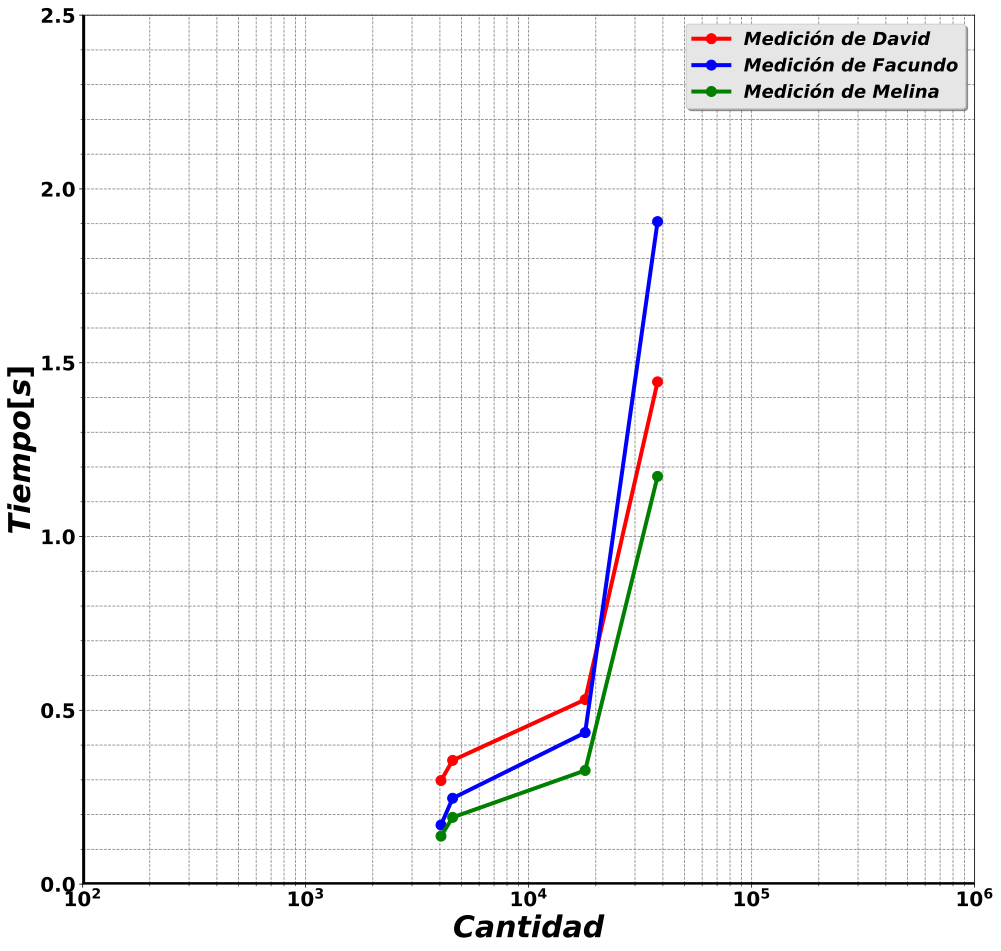
\includegraphics[width = 0.65\textwidth]{graficos_mediciones/medicionesLineas}
%    \caption{Gráfico Cantidad de Líneas vs. Tiempo}
%    \label{fig:medicionesLineas}
%\end{figure}

\newpage

\section{Bibliografía}
\newpage

\section{Código fuente}
\begin{lstlisting}
#include <stdio.h>
#include <stdlib.h>
#include <string.h>

#define error_cant_param "Cantidad incorrecta de argumentos"
#define error_param_incorrectos "Las opciones ingresadas son incorrectas"
#define error_archivo_inexistente "El archivo que intenta abrir no existe"
#define mensaje_de_ayuda "Usage:\n \ttp0 -h\n\ttp0 -V\n\ttp0 [options] file\nOptions:\n\t-V, --version\t\tPrint version and quit.\n\t-h, --help\t\tPrint this information.\n\t-l, --lines\t\tPrint number of lines in file.\n\t-w, --words\t\tPrint number of words in files.\n\t-c, --characters\tPrint number of characters in file.\n\t-i, --input\t\tPath to input file.\nExamples:\n\n\ttp0 -w -i input.txt"
#define version_num "tp0 v1.0"

// Muestra ayuda
void ayuda()
{
    printf("%s\n",mensaje_de_ayuda);
}

// Muestra la versión del programa
void version()
{
    printf("%s\n",version_num);
}

// Muestra error y termina ejecucion
void error(char *mensaje)
{
    fprintf(stderr,"%s\n",mensaje);
    // fprintf se usa para escribir en stderr
    exit(0);
    // exit termina la ejecucion del programa
}
\end{lstlisting}


\begin{verbatim}
    #include <stdio.h>
#include <stdlib.h>
#include <string.h>

#define error_cant_param "Cantidad incorrecta de argumentos"
#define error_param_incorrectos "Las opciones ingresadas son incorrectas"
#define error_archivo_inexistente "El archivo que intenta abrir no existe"
#define mensaje_de_ayuda "Usage:\n \ttp0 -h\n
\ttp0 -V\n\ttp0 [options] file\nOptions:\n
\t-V, --version\t\tPrint version and quit.\n
\t-h, --help\t\tPrint this information.\n
\t-l, --lines\t\tPrint number of lines in file.\n
\t-w, --words\t\tPrint number of words in files.\n
\t-c, --characters\tPrint number of characters in file.\n
\t-i, --input\t\tPath to input file.\n
Examples:\n\n\ttp0 -w -i input.txt"
#define version_num "tp0 v1.0"

// Muestra ayuda
void ayuda(){
    printf("%s\n",mensaje_de_ayuda);
}

// Muestra la versión del programa
void version(){
    printf("%s\n",version_num);
}

// Muestra error y termina ejecución
void error(char *mensaje){
    fprintf(stderr,"%s\n",mensaje);
    // fprintf se usa para escribir en stderr
    exit(0);
    // exit termina la ejecución del programa
}
\end{verbatim}
\newpage

\begin{verbatim}
char * string_token(char *str,const char *delim,char **temp)
{
    register char *tok;

    if(str!=NULL)
    {
        for(tok=str;*tok;tok++)
            if(strchr(delim,*tok)!=NULL)
                break;
            if(!(*tok))
                *temp=tok;
            else{
                *tok='\0';
                *temp=tok+1;
            }
    }else{
		if(!(**temp))
			return NULL;
		str=*temp;
		for(tok=str;*tok;tok++)
			if(strchr(delim,*tok)!=NULL)
				break;

		if(!(*tok)){
			*temp=tok;
			return str;
		}else{
			*tok='\0';
			*temp=tok+1;
		}
	}
	return str;
}
\end{verbatim}
\newpage

\begin{verbatim}
char * clone_string (const char * orig)
{
	size_t len=0;
	size_t i=0;
    char * clone=NULL;

	if(orig==NULL )
		NULL;

	len=strlen(orig);

	if((clone=(char *)malloc(sizeof(char)*(len+1)))==NULL)
		NULL;
	
	for(i=0;i<=len;i++)
		clone[i]=orig[i];

	return clone;
}

void destroy_string (char *str){

	if(str==NULL)
		return;
	free(str);
	return;
}

void destroy_string_array(char **str_arr, size_t len)
{
	size_t i=0;

	if(str_arr==NULL)
		return;

	for(i = 0; i < len; i++)
	{
		free(str_arr[i]);
		str_arr[i] = NULL;
	}
	free(str_arr);
	str_arr=NULL;
	return;
}
\end{verbatim}
\newpage

\begin{verbatim}
char ** split_string(char * str,char * delim, size_t *len)
{
	char *dup, *q, *p,*temp;
	size_t n, i;
    char ** str_arr;

	if(str==NULL || delim==NULL || len==NULL)
		return NULL;

	if((dup=clone_string(str))==NULL)
		return NULL;

	for(n=0,i=0;dup[i];i++)
		if(strchr(delim,dup[i])!=NULL)
			n++;

	if((str_arr=(char **)malloc(sizeof(char*)*(n+1)))==NULL){
		destroy_string(dup);
		*len=0;
		return NULL;
	}
	for(i=0,q=dup;(p= string_token(q,delim,&temp))!=NULL;q=NULL,i++)
	{
		if((str_arr[i] =clone_string(p)) ==NULL)
		{
			destroy_string_array(str_arr, i);
			destroy_string(dup);
			*len=0;
			return NULL;
		}
	}
	destroy_string(dup);
	*len=i;
	return str_arr;
}
\end{verbatim}
\newpage

\begin{verbatim}
// Cuenta caracteres
int contar_caracteres(FILE *archivo){

    char ch;
    int contador = 0;

    while ((ch = fgetc(archivo)) != EOF){
        if ((ch != '\n') || (ch != ' ') || (ch != '\t') || (ch != '\0'))
            contador++;
    }

    fclose(archivo);
    return contador;
}

// Cuenta palabras
int contar_palabras(FILE *archivo){
    char linea[100 + 1];
    int i, cantidad_palabras = 0;
    char ** string_array=NULL;
    size_t len=0;
    char *delim= " \t\n\r";

    while (fgets(linea, 300, archivo) != NULL) {
        string_array=split_string(linea,delim, &len);
        for(i=0;i<len;i++){
            if(strlen(string_array[i])>0)
            cantidad_palabras++;
        }
    destroy_string_array(string_array,len);
    len=0;           
    }    

    return cantidad_palabras;
}
\end{verbatim}
\newpage

\begin{verbatim}
// Cuenta líneas
int contar_lineas(FILE *archivo){
    
    char ch;
    int contador = 0;

    while ((ch = fgetc(archivo)) != EOF){
        if (ch == '\n'){
            contador++;
        }

    }

    fclose(archivo);
    return contador;
}
\end{verbatim}
\newpage

\begin{verbatim}
int main(int argc, char *argv[]){
//argc -> argument count, argv -> argument vector

    // Puntero a archivo
    FILE *file;

    // Verifica la cantidad de argumentos
    if (argc < 2 || argc > 4){
        error(error_cant_param);
    }

    // Verifica por pedido de ayuda en el primer argumento
    else if ((strcmp(argv[1], "-h") == 0) || 
             (strcmp(argv[1], "--help") == 0)){
        // Por si hay algo luego del pedido de ayuda
        if (argc != 2) error(error_cant_param);
        ayuda();
        return 0;
    }

    // Verifica por pedido de versión en el primer argumento
    else if ((strcmp(argv[1], "-V") == 0) || 
             (strcmp(argv[1], "--version") == 0)){
        // Por si hay algo luego del pedido de versión
        if (argc != 2) error(error_cant_param);
        version();
        return 0;
    }

    // Verifica por pedido de caracteres en el primer argumento 
    // y entrada en el segundo argumento
    else if (((strcmp(argv[1], "-c") == 0) || 
              (strcmp(argv[1], "--characters") == 0)) && 
             ((strcmp(argv[2], "-i") == 0) || 
              (strcmp(argv[2], "--input") == 0))){
        // Por si hay algo luego del nombre del archivo
        if (argc != 4) error(error_cant_param);

        // Se intenta abrir el archivo en modo lectura
        file = fopen(argv[3], "r");
        if (file == NULL) error(error_archivo_inexistente);

        int num;
        num = contar_caracteres(file);
        printf("%d %s\n", num, argv[3]);
        return 0;
    }

    // Verifica por pedido de palabras en el primer argumento 
    // y entrada en el segundo argumento
    else if (((strcmp(argv[1], "-w") == 0) || 
              (strcmp(argv[1], "--words") == 0)) && 
             ((strcmp(argv[2], "-i") == 0) || 
              (strcmp(argv[2], "--input") == 0))){
        // Por si hay algo luego del nombre del archivo
        if (argc != 4) error(error_cant_param);

        // Se intenta abrir el archivo en modo lectura
        file = fopen(argv[3], "r");
        if (file == NULL) error(error_archivo_inexistente);

        int num;
        num = contar_palabras(file);
        printf("%d %s\n", num, argv[3]);
        return 0;
    }

    // Verifica por pedido de líneas en el primer argumento 
    // y entrada en el segundo argumento
    else if (((strcmp(argv[1], "-l") == 0) || 
              (strcmp(argv[1], "--lines") == 0)) && 
             ((strcmp(argv[2], "-i")) || 
              (strcmp(argv[2], "--input")))){
        // Por si hay algo luego del nombre del archivo
        if (argc != 4) error(error_cant_param);

        // Se intenta abrir el archivo en modo lectura
        file = fopen(argv[3], "r");
        if (file == NULL) error(error_archivo_inexistente);

        int num;
        num = contar_lineas(file);
        // Se convierte num a decimal
        printf("%d %s\n", num, argv[3]);
        return 0;
    }     

    // Opciones ingresadas incorrectas
    else {
        error(error_param_incorrectos);
    }

    return 0;
}
\end{verbatim}



\end{document}